\documentclass[11pt,onecolumn,twoside]{style_tp}

\newif\ifVIEWALL
\VIEWALLfalse %Ne pas afficher le contenu pour le prof
%\VIEWALLtrue %Afficher tout le contenu (prof + eleve)
%\VIEWALLTOCHOOSE

%Le r\'epertoire contenant les ressources
\def\repRessource{ressources}

%Le repertoire contenant les listings
\def\repList{ressources/listings}

%Le fichier contenant toutes les d\'efinitions des macros
%%%%%%%%%%%%%%%%%%%%%%%%%%%%%%%%%%%%%%%%%%%%%%%%%%%%%%%%%%%%%%%%%%%%%%%%%%%%%%%%%%%%%%%%%%%%%%%%
%%%%%%%%%%%%%%%%%%%%%%%%%%%%%%%%%%%%%%%%%%%%%%%%%%%%%%%%%%%%%%%%%%%%%%%%%%%%%%%%%%%%%%%%%%%%%%%%
%\usepackage{pdfsync}
%\usepackage{hyperlatex}
\usepackage[utf8]{inputenc}
\usepackage{lmodern}
\usepackage[french]{babel}
\usepackage[T1]{fontenc}
\usepackage{verbatim}
\usepackage{xcolor}
\definecolor{linkcol}{rgb}{0.06,0.06,0.6}
\definecolor{citecol}{rgb}{0.6,0.04,0.04}
\definecolor{red}{rgb}{0.6,0.04,0.04}
\definecolor{blue}{rgb}{0.06,0.06,0.6}
\definecolor{grey}{rgb}{0.4,0.4,0.4}
\newcommand{\empha}[1]{\textbf{\textcolor{blue}{#1}}}
\newcommand{\emphb}[1]{\textcolor{red}{#1}}
\newcommand{\colorSection}{blue}
\newcommand{\colorSubSection}{blue}
\newcommand{\colorSubSubSection}{blue}
\newcommand{\colorChapter}{blue}

%Les chemins o\`u se trouvent les figures et les extensions de figures
% My pdf code
\usepackage{ifpdf}
\ifpdf
  \usepackage[pdftex]{graphicx}
  \DeclareGraphicsExtensions{.jpg,.pdf,.png}
  \usepackage[pagebackref,hyperindex=true,linktoc=all]{hyperref}
\else
  \usepackage{graphicx}
  \DeclareGraphicsExtensions{.ps,.eps}
  \usepackage[dvipdfm,pagebackref,hyperindex=true,linktocpage]{hyperref}
\fi
\hypersetup
{
pdfauthor="Olivier COTS", %auteur du document
pdfstartview={XYZ null null 1},
pdfhighlight=/O, %effet d'un clic sur un lien hypertexte
colorlinks=true, %couleurs sur les liens hypertextes
linkcolor=linkcol, %couleur des liens hypertextes internes
citecolor=citecol, %couleur des liens pour les citations
urlcolor=linkcol %couleur des liens pour les url
}
%\usepackage{graphicx}
\graphicspath{{\repRessource/figures/}}

%Les marges
\usepackage[a4paper,includeheadfoot,margin=2.54cm]{geometry}

%Hampath website
\newcommand{\homepage}{http://cots.perso.enseeiht.fr}
\newcommand{\resources}{\homepage/resources}

%Les maths et ams
\usepackage{amsfonts}
\usepackage{amscd}
\usepackage{amsthm}
\usepackage{amsmath}
\usepackage{amssymb}
\usepackage{mathrsfs}
\usepackage{mathtools}
\usepackage{xstring}
\usepackage{dsfont}

%Theorem style
%%-------------------
%\theoremstyle{plain}
%%-------------------
%\newtheorem{thrm}{Theorem}[section]
%\newtheorem{lmm}[thrm]{Lemma}
%\newtheorem{crllr}[thrm]{Corollary}
%\newtheorem{prpstn}[thrm]{Proposition}
%\newtheorem{crtrn}[thrm]{Criterion}
%\newtheorem{lgrthm}[thrm]{Algorithm}
%%------------------------
%\theoremstyle{definition}
%%------------------------
%\newtheorem{dfntn}[thrm]{Definition}
%\newtheorem{cnjctr}[thrm]{Conjecture}
%\newtheorem{xmpl}[thrm]{Example}
%\newtheorem{prblm}[thrm]{Problem}
%\newtheorem{rmrk}[thrm]{Remark}
%\newtheorem{nt}[thrm]{Note}
%\newtheorem{clm}[thrm]{Claim}
%\newtheorem{smmr}[thrm]{Summary}
%\newtheorem{cs}[thrm]{Case}
%\newtheorem{bsrvtn}[thrm]{Observation}
%
% Definitions des environnements des theoremes,...
%-------------------
\newtheoremstyle{mystyleTheorem}%       % Name
  {}%                                     % Space above
  {}%                                     % Space below
  {\itshape}%                             % Body font
  {}%                                     % Indent amount
  {}%                            % Theorem head font
  {.}%                                    % Punctuation after theorem head
  { }%                                    % Space after theorem head, ' ', or \newline
%  {}%                                     % Theorem head spec (can be left empty, meaning `normal')
  {\noindent\textbf{\thmname{#1}\thmnumber{~#2}}\thmnote{\color{blue}~(#3)}}%

\newtheoremstyle{mystyleDefinition}%       % Name
  {}%                                     % Space above
  {}%                                     % Space below
  {}%                             % Body font
  {}%                                     % Indent amount
  {}%                            % Theorem head font
  {.}%                                    % Punctuation after theorem head
  { }%                                    % Space after theorem head, ' ', or \newline
%  {}%                                     % Theorem head spec (can be left empty, meaning `normal')
  {\noindent\textbf{\thmname{#1}\thmnumber{~#2}}\thmnote{\color{blue}~(#3)}}%

\theoremstyle{mystyleTheorem}
%-------------------
\newtheorem{theorem}{Th\'eor\`eme}[chapter]         % Theoreme
\newtheorem{proposition}[theorem]{Proposition}      % Proposition
\newtheorem{lemma}[theorem]{Lemme}                  % Lemme
\newtheorem{cor}[theorem]{Corollaire}               % Corollaire d'un theoreme
%---------------------------------------------------------
%\newtheorem{question}{Question}                     % Question
\newtheorem{difficulty}{Difficult\'e}               % Difficult\'e
%------------------------

\theoremstyle{mystyleDefinition}
%------------------------
\newtheorem{definition}{D\'efinition}[chapter]      % Definition
%
\newtheorem{example}{Exemple}[chapter]              % Exemple
\newtheorem{counterexample}[example]{Contre-exemple}% Contre Exemple
\newtheorem{exercice}[example]{Exercice}            % Exercice
%
\newtheorem{assumption}{Hypoth\`ese}[chapter]       % Hypoth\`ese
%------------------------
\theoremstyle{remark}
%------------------------
\newtheorem{remark}{Remarque}[chapter]              % Remarque

%%%% Environnement pour les exercices %%%%%%%%%%%%%%%%%%%%%%%%%%%%%%%%%%%%%%%
%% \theoremstyle{plain}
\theoremstyle{mystyleDefinition}
\newtheorem{Exercice}{{\makebox[0pt][r]{$\rhd$\hspace*{1ex}}Exercice}}[chapter]
\newtheorem{Question}{Question}%[Exercice]
\newtheorem{SousQuestion}{\hspace*{1em}}[Question]
\newtheorem{Exemple}{Exemple}
\newcounter{exercice}
\newcounter{question}[exercice]
\renewcommand{\theexercice}{\arabic{exercice}}
\renewcommand{\thequestion}{\theexercice.\arabic{question}}
\theoremstyle{definition}
\newtheorem{Guide}{{\makebox[0pt][r]{$\blacktriangleright$\hspace*{1ex}}Guide}}
\renewcommand{\theGuide}{\hspace*{-0.9ex}}

%Tag \`a gauche ou \`a droite
\makeatletter
\newcommand{\reqnomode}{\tagsleft@false\let\veqno\@@eqno}
\newcommand{\leqnomode}{\tagsleft@true\let\veqno\@@leqno}
\makeatother

%Exigences
\reversemarginpar
%\newcommand{\attB}{\textcolor{green}{\textbullet}}
%\newcommand{\attM}{\textcolor{green}{\textbullet}\textcolor{orange}{\textbullet}}
%\newcommand{\attH}{\textcolor{green}{\textbullet}\textcolor{orange}{\textbullet}\textcolor{red}{\textbullet}}
\newcommand{\anoter}{ {\Large \textcolor{orange}{\ding{45}}} }

%Elements differentiel
%\newcommand{\diff}{\mathop{}\mathopen{}\mathrm{d}}
\newcommand{\xDif}{{\rm D}}
\newcommand{\xdif}{\,{\rm d}}
\newcommand{\diff}{\xdif}
\newcommand{\Diff}{{\rm \partial}}

%Les ensembles
%\newcommand{\U}{\mbox{$\mathbf{U}$}\xspace}
%\newcommand{\X}{\mbox{$\mathbf{X}$}\xspace}
%\newcommand{\M}{\mbox{$\mathbf{M}$}\xspace}
\newcommand{\U}{U}
\newcommand{\X}{X}
%\newcommand{\M}{M}
\newcommand{\Lcal}{\mathcal{L}}
\newcommand{\Ucal}{\mathcal{U}}
\newcommand{\I}{\mathcal{I}}
\newcommand{\A}{\mathcal{A}}
\renewcommand{\O}{\mathcal{O}}
\newcommand{\B}{\mathcal{B}}
\newcommand{\E}{\mathcal{E}}
\newcommand{\F}{\mathcal{F}}
\newcommand{\D}{\mathcal{D}}
\renewcommand{\P}{\mathcal{P}}
\newcommand{\V}{\mathcal{V}}
\newcommand{\xLn}[1]{{\rm L}^#1}
\newcommand{\xCn}[1]{{\rm C}^#1}

%Les softs et librairies
\newcommand{\pcr}[1]{{\fontfamily{pcr}\selectfont #1}}
%\newcommand{\vrb}[1]{{\fontfamily{ttfamily}\selectfont #1}}
\newcommand{\vrb}[1]{\texttt{#1}}
\newcommand{\cmd}[1]{\texttt{#1}}
\newcommand{\lib}[1]{\textsc{#1}}
\newcommand{\hampath}{\texttt{HamPath}}
\newcommand{\cotcot}{\texttt{cotcot}}
\newcommand{\matlab}{\lib{Matlab}}
\newcommand{\octave}{\lib{Octave}}
\newcommand{\fortran}{\lib{Fortran}}
\newcommand{\python}{\lib{Python}}
\newcommand{\interface}{\lib{Interface}}

%Intervalle
\newcommand{\intervalle}[4]{\mathopen{#1}#2
                                \mathclose{}\mathpunct{},#3
                                \mathclose{#4}}
\newcommand{\intervalleff}[2]{\intervalle{[}{#1}{#2}{]}}
\newcommand{\intervalleof}[2]{\intervalle{]}{#1}{#2}{]}}
%\newcommand{\intervalleof}[2]{\intervalle{(}{#1}{#2}{]}}
\newcommand{\intervallefo}[2]{\intervalle{[}{#1}{#2}{[}}
%\newcommand{\intervallefo}[2]{\intervalle{[}{#1}{#2}{)}}
\newcommand{\intervalleoo}[2]{\intervalle{]}{#1}{#2}{[}}
%\newcommand{\intervalleoo}[2]{\intervalle{(}{#1}{#2}{)}}
\newcommand{\intervalleentier}[2]{\intervalle{\llbracket}{#1}{#2}{\rrbracket}}

%L'arc de cercle pour les champs de Jacobi
\usepackage{yhmath}

%Misc
\newcommand\ie{\textit{i.e. }}
\newcommand\cf{\textit{cf. }}
\newcommand{\myemph}[1]{\textit{#1}}
\newcommand{\refcite}[1]{r\'ef.~\cite{#1}}
\newcommand{\refscite}[1]{r\'efs.~\cite{#1}}
\newcommand{\figsref}[1]{figs.~\ref{#1}}
\newcommand{\figref}[1]{fig.~\ref{#1}}
\newcommand{\frp}[2]{\frac{\Diff #1}{\Diff #2}}
\newcommand{\frpp}[2]{{\Diff #1}/{\Diff #2}}

%La commande pour la todo_list
\newcommand{\todo}[1]{\noindent {\color{red} \it TODO!!! #1}~\\}

%Ensembles de nombres
\newcommand{\nbSet}[1]{\mathbb{#1}}
\newcommand{\setPositive}{\text{\bf{\tiny+}}}
\newcommand{\setNegative}{\mathbb{\tiny-}}
\newcommand{\setStar}{\text{*}}
\newcommand{\M}{\nbSet{M}}
\newcommand{\N}{\nbSet{N}}
\newcommand{\Z}{\nbSet{Z}}
\newcommand{\Q}{\nbSet{Q}}
\newcommand{\R}{\nbSet{R}} %\newcommand{\R}{\mathbb{R}}
\newcommand{\C}{\nbSet{C}}


\newcommand{\setDeco}[2]{
    \IfEqCase{#2}{
        {s}{\nbSet{#1}^{\setStar}}
        {n}{\nbSet{#1}^{\phantom{\setStar}}_{\setNegative}}
        {p}{\nbSet{#1}^{\phantom{\setStar}}_{\setPositive}}
        {sn}{\nbSet{#1}^{\setStar}_{\setNegative}}
        {sp}{\nbSet{#1}^{\setStar}_{\setPositive}}
    }
}

\newcommand{\Ns}{ \ensuremath{\setDeco{N}{s}} }
\newcommand{\Rn}{ \ensuremath{\setDeco{R}{n}} }
\newcommand{\Rp}{ \ensuremath{\setDeco{R}{p}} }
\newcommand{\Rs}{ \ensuremath{\setDeco{R}{s}} }
\newcommand{\Rsp}{ \ensuremath{\setDeco{R}{sp}} }
\newcommand{\Rsn}{ \ensuremath{\setDeco{R}{sn}} }

%Valeur absolue et norme
\newcommand{\abs}[1]{\lvert#1\rvert} 
\newcommand{\absStyle}[1]{\left\lvert#1\right\rvert}
\newcommand{\norme}[1]{\lVert#1\rVert}
\newcommand{\normeStyle}[1]{\left\lVert#1\right\rVert}

%Petit o et grand O
\newcommand{\petito}[1]{o\mathopen{}\left(#1\right)}
\newcommand{\grandO}[1]{O\mathopen{}\left(#1\right)}

%Ensemble des .. tels que ..
\newcommand{\enstq}[2]{\left\{#1\mathrel{}\middle|\mathrel{}#2\right\}}

%Produit scalaire
\newcommand{\prodscal}[2]{\left(#1 \,|\, #2\right)}
\newcommand{\crochetDualite}[2]{\left\langle#1,#2\right\rangle}

%Fl\`eche
\usepackage[f]{esvect}
%\newcommand\vvec{\vec}
\newcommand\vvec{\overrightarrow}
\renewcommand\tilde{\widetilde}

%Solutions du PMP
\newcommand\lsol{\bar{\lambda}}
\newcommand\xsol{\bar{x}}
\newcommand\ysol{\bar{y}}
\newcommand\usol{\bar{u}}
\newcommand\zsol{\bar{z}}
\newcommand\psol{\bar{p}}
\newcommand\tfsol{\bar{t}_f}
\newcommand\tsol{\bar{t}\hspace{0.1em}}

% Lettres avec tilde
\def\xt{\widetilde{x}}
\def\ut{\widetilde{u}}
\def\pt{\widetilde{p}}
\def\ft{\widetilde{f}}

%Op\'erateur math
\DeclareMathOperator{\argmax}{arg\,max}
%\DeclareMathOperator{\rank}{rank}
\DeclareMathOperator{\codim}{codim}
\DeclareMathOperator{\rang}{rang}
\DeclareMathOperator{\rank}{rang}
\DeclareMathOperator{\vect}{Vect}
\DeclareMathOperator{\Isom}{Isom}
\DeclareMathOperator{\im}{Im}
\DeclareMathOperator{\supp}{supp}
\DeclareMathOperator{\sign}{sign}
\DeclareMathOperator{\comp}{num}

%exponential mapping
\newcommand{\expmap}[3]{\exp({#2 #3}) (#1)}

%Fonction homotopique
\renewcommand{\hom}{\Phi}

%Epsilon, phi, theta, etc.
\newcommand{\veps}{\varepsilon}
\newcommand\vphi{\phi}
\newcommand\pth{p_\theta}
\renewcommand\th{\theta}

\newcommand{\arc}{\gamma}

%Les dessins
\usepackage{tikz}
\usepackage{pgfkeys}
\usepackage{circuitikz}
\usetikzlibrary{arrows,shapes,backgrounds,patterns}
\usepackage{pifont}
\usepackage{tikzgraphicx}
\tikzstyle{every picture}+=[remember picture]
\tikzstyle{na} = [baseline=-.5ex]
\makeatletter
\newcommand{\gettikzxy}[3]{%
  \tikz@scan@one@point\pgfutil@firstofone#1\relax
  \edef#2{\the\pgf@x}%
  \edef#3{\the\pgf@y}%
}
\makeatother

% Définition des nouvelles options xmin, xmax, ymin, ymax
% Valeurs par défaut : -3, 3, -3, 3
\tikzset{
    xmin/.store in=\xmin, xmin/.default=-3, xmin=-3,
    xmax/.store in=\xmax, xmax/.default=3, xmax=3,
    ymin/.store in=\ymin, ymin/.default=-3, ymin=-3,
    ymax/.store in=\ymax, ymax/.default=3, ymax=3,
}
% Commande qui trace la grille entre (xmin,ymin) et (xmax,ymax)
\newcommand {\grille}
    {\draw[help lines] (\xmin,\ymin) grid (\xmax,\ymax);}
% Commande \axes
\newcommand {\axes}[2] {
    \draw[->,gray] (\xmin,0) -- (\xmax,0);
    \draw[->,gray] (0,\ymin) -- (0,\ymax);
    \draw (\xmax,0) node[below]{#1};
    \draw (0,\ymax) node[left]{#2};
}
% Commande qui limite l’affichage à (xmin,ymin) et (xmax,ymax)
\newcommand {\fenetre}
    {\clip (\xmin,\ymin) rectangle (\xmax,\ymax);}

%Les tableaux
\usepackage{calc}
\usepackage{array}
\newcolumntype{C}[1]{>{\centering}p{#1}}
\newcolumntype{L}[1]{>{\raggedright}p{#1}}

%Tableau : \'epaisseur des lignes
\usepackage{booktabs}
\newcommand{\smallhrule}{\specialrule{0.02em}{0.25em}{0.25em}}
\newcommand{\medhrule}{\specialrule{0.05em}{0.3em}{0.3em}}
\newcommand{\bighrule}{\specialrule{0.1em}{0.3em}{0.5em}}

%Passage seulement pour la version prof
\newcommand{\noi}{\noindent}
\newcommand{\HRule}{\noi\rule{\linewidth}{0.3mm}}
\newcommand{\onlyForProf}[1]{
\ifVIEWALL
    {
    \newpage
    {\color{grey}
        \noindent\fbox{\parbox{\linewidth-2\fboxrule-2\fboxsep}{\centering \textbf{Remarques personnelles}}}
        ~\\
        #1
        ~\\
        \HRule
    }
    \newpage
    } \else
\fi}

%Pour avoir des notes dans la marge
\newcommand{\noteInMarge}[1]{\ifVIEWALL{ \marginpar{{\color{red} #1}} }\else\fi}


%-------------------------------------------------------------------------------------------------------------------------------
%-------------------------------------------------------------------------------------------------------------------------------
%Pour le style du manuscrit

\usepackage{fancyhdr}                    % Fancy Header and Footer
\usepackage{colortbl}

% Clear Header Style on the Last Empty Odd pages
\makeatletter
\def\cleardoublepage{
    \clearpage
    \if@twoside 
        \ifodd
            \c@page
        \else%
            \hbox{}%
            \thispagestyle{empty}%              % Empty header styles
            \newpage%
            \if@twocolumn\hbox{}\newpage
            \fi
        \fi
    \fi}
\makeatother

%minitoc
%\usepackage[nottoc, notlof, notlot]{tocbibind}
\usepackage[french]{minitoc}
\setcounter{minitocdepth}{2}
\setlength{\mtcindent}{18pt} 
\renewcommand{\mtcfont}{\small\rm} 
\renewcommand{\mtcSfont}{\small\bf}

%\let\minitocORIG\minitoc
%\renewcommand{\minitoc}{\minitocORIG \vspace{1.5em}}

%table des mati\`eres et compteurs de titres
\setcounter{secnumdepth}{4}
\setcounter{tocdepth}{2}

% centered page environment
\newenvironment{vcenterpage}
{\newpage\vspace*{\fill}\thispagestyle{empty}\renewcommand{\headrulewidth}{0pt}}
{\vspace*{\fill}}

%nicer backref links
\renewcommand*{\backref}[1]{}
\renewcommand*{\backrefalt}[4]{%
\ifcase #1 %
%
\or
$\hookleftarrow$~#2.%
\else
$\hookleftarrow$~#2.%
\fi}
\renewcommand*{\backrefsep}{, }
\renewcommand*{\backreftwosep}{ et~}
\renewcommand*{\backreflastsep}{ et~}
%-------------------------------------------------------------------------------------------------------------------------------
%-------------------------------------------------------------------------------------------------------------------------------

%------------------------------------------------------------------------------------------------------------%
%Compteur pour les probl\`emes
\usepackage{totcount}
\newcounter{problem}%[chapter]
\regtotcounter{problem}
\newcommand{\tagProblem}[1][]{%
    \addtocounter{problem}{1}
    \tag{P\theproblem#1}
    %\tag{P\thechapter.\theproblem#1}
}
%Compteur pour les hypoth\`eses
\newcounter{assumptionx}[chapter]
\regtotcounter{assumptionx}
\newcommand{\tagAssumption}{%
    H\thechapter.\theassumptionx
}

\newenvironment{myassumption}
{\addtocounter{assumptionx}{1}
 \renewcommand\theassumption{\tagAssumption}
 \addtocounter{assumption}{-1}
 \begin{flushleft}
 \begin{tabular}{|| L{0.94\textwidth}}
  \assumption
  \vspace{-1em}
}
{\vspace{-1em}
\endassumption
\end{tabular}
 \end{flushleft}
 }

% \newenvironment{myassumption}{
%    \begin{flushright}
%        \begin{tabular}{|| L{0.94\textwidth} }
%            %\begin{assumption}
%            \textbf{Hypoth\`ese \tagAssumption.}
%            %\vspace{-1em}
%    }
%    {
%            %\vspace{-1em}
%            %\end{assumption}
%        \end{tabular}
%    \end{flushright}
%}

%Remarque perso
%\newcommand{\myremark}[1]{
%    \begin{flushright}
%        \begin{tabular}{| L{0.94\textwidth} }
%            \begin{remark}
%            \vspace{-1em}
%                #1
%            \vspace{-1em}
%            \end{remark}
%        \end{tabular}
%    \end{flushright}
%}
\newenvironment{myremark}{
    \begin{flushright}
        \begin{tabular}{| L{0.94\textwidth} }
            \begin{remark}
            \vspace{-1em}
    }
    {
            \vspace{-1em}
            \end{remark}
        \end{tabular}
    \end{flushright}
}

\newenvironment{myQuestion}{
    \begin{flushright}
        \begin{tabular}{| L{0.94\textwidth} }
            \begin{Question}
            \vspace{-1em}
    }
    {
            \vspace{-1em}
            \end{Question}
        \end{tabular}
    \end{flushright}
}

\newenvironment{myExercice}{
    \begin{flushright}
        \begin{tabular}{| L{0.94\textwidth} }
            \begin{Exercice}
            \vspace{-1em}
    }
    {
            \vspace{-1em}
            \end{Exercice}
        \end{tabular}
    \end{flushright}
}

%%%%%%%%%%%%%%%%%%%%%%%%%%%%%%%%%%%%%%%%
\usepackage[many]{tcolorbox}% http://ctan.org/pkg/tcolorbox
%\definecolor{mycolor}{rgb}{0.2,0.4,0.6}% Rule colour
%\definecolor{mycolor}{rgb}{0.122, 0.435, 0.698}% Rule colour
\makeatletter
%\newcommand{\myfbox}[2]{%
%  \setbox0=\hbox{#2}%
%  %\setlength{\@tempdima}{\dimexpr\wd0+13pt}%
%  \setlength{\@tempdima}{#1\textwidth}%
%  \begin{tcolorbox}[colframe=mycolor,boxrule=0.5pt,arc=4pt,
%      left=6pt,right=6pt,top=6pt,bottom=6pt,boxsep=0pt,width=\@tempdima]
%    #2
%  \end{tcolorbox}
%}
\newcommand{\myfbox}[4][]{%
%  \setbox0=\hbox{#3}%
    \setlength{\@tempdima}{#2\textwidth}%
    %\begin{tcolorbox}[colback=#3!2!white,colframe=#3,boxrule=0.5pt,arc=4pt,left=6pt,right=6pt,
    \begin{tcolorbox}[colback=white,colframe=#3,boxrule=0.8pt,arc=6pt,left=6pt,right=6pt,
          top=6pt,bottom=6pt,boxsep=0pt,width=\@tempdima,#1]
        #4
    \end{tcolorbox}
}
\makeatother

%\newcommand{\envbox}[2][theorem]{%
%    \begin{center}
%    \begin{minipage}[h!]{0.98\textwidth}
%        \myfbox{1.0}{blue}{
%        \begin{#1}
%            #2
%        \end{#1}
%        }
%    \end{minipage}
%    \end{center}
%}

\usepackage{xargs}
\newcommandx{\envbox}[3][1=theorem,2=]{%
    \begin{center}
    \begin{minipage}[h!]{0.999\textwidth}
        \myfbox{1.0}{blue}{
        \begin{#1}[#2]
            #3
        \end{#1}
        }
    \end{minipage}
    \end{center}
}

%Pr\'erequis
\newcommand{\prerequis}[1]{
%    \noindent\fbox{\parbox{\linewidth-2\fboxrule-2\fboxsep}{\textbf{Pr\'e-requis :} #1}}
%    \vspace{0.5em}
    \begin{center}
    \begin{minipage}[h!]{0.98\textwidth}
        \myfbox{1.0}{gray}{
        \textbf{Pr\'e-requis :} #1
        }
    \end{minipage}
    \end{center}
}

%%%%%%%%%%%%%%%%%%%%%%%%%%%%%%%%%%%%%%%%

%Proof
\makeatletter
\renewenvironment{proof}[1][\proofname]{
    \par\pushQED{\qed}\small\normalfont\topsep6\p@\@plus6\p@\relax\trivlist\item[\hskip\labelsep\itshape#1\@addpunct{.}]\ignorespaces
}{
    \popQED\endtrivlist\@endpefalse
}
\makeatother

%Les itemize
\usepackage{marvosym}
\usepackage{enumitem}
\frenchbsetup{CompactItemize=false}
\setlist{itemsep=0.25em}
\setitemize[1]{label={\small \Football}}
\setitemize[2]{label=$\diamond$}

\newcommand*\circled[1]{\tikz[baseline=(char.base)]{
    \node[shape=circle,draw,inner sep=2pt] (char) {#1};}}

\newcommand{\pgftextcircled}[1]{
    \setbox0=\hbox{#1}%
    \dimen0\wd0%
    \divide\dimen0 by 2%
    \begin{tikzpicture}[baseline=(a.base)]%
        \useasboundingbox (-\the\dimen0,0pt) rectangle (\the\dimen0,1pt);
        \node[circle,draw,outer sep=0pt,inner sep=0.1ex] (a) {#1};
    \end{tikzpicture}
}

%Les enumerations
%\usepackage{enumerate}

\usepackage{listings}
\definecolor{mymauve}{rgb}{0.58,0,0.82}
\lstset{ %
  backgroundcolor=\color{white},   % choose the background color; you must add \usepackage{color} or \usepackage{xcolor}
  basicstyle=\small,               % the size of the fonts that are used for the code
  breakatwhitespace=false,         % sets if automatic breaks should only happen at whitespace
  breaklines=true,                 % sets automatic line breaking
  captionpos=b,                    % sets the caption-position to bottom
  commentstyle=\color{blue},       % comment style
  deletekeywords={...},            % if you want to delete keywords from the given language
  escapeinside={\%*}{*)},          % if you want to add LaTeX within your code
  extendedchars=true,              % lets you use non-ASCII characters; for 8-bits encodings only, does not work with UTF-8
  frame=single,                    % adds a frame around the code
  keepspaces=true,                 % keeps spaces in text, useful for keeping indentation of code (possibly needs columns=flexible)
  keywordstyle=\color{red},        % keyword style
  otherkeywords={*,...},           % if you want to add more keywords to the set
  numbers=none,                    % where to put the line-numbers; possible values are (none, left, right)
  numbersep=5pt,                   % how far the line-numbers are from the code
  numberstyle=\tiny\color{gray},   % the style that is used for the line-numbers
  rulecolor=\color{black},         % if not set, the frame-color may be changed on line-breaks within not-black text (e.g. comments (green here))
  showspaces=false,                % show spaces everywhere adding particular underscores; it overrides 'showstringspaces'
  showstringspaces=false,          % underline spaces within strings only
  showtabs=false,                  % show tabs within strings adding particular underscores
  stepnumber=2,                    % the step between two line-numbers. If it's 1, each line will be numbered
  stringstyle=\color{mymauve},     % string literal style
  tabsize=2,                       % sets default tabsize to 2 spaces
  %title=\lstname,                 % show the filename of files included with \lstinputlisting; also try caption instead of title
  frameround=tttt                  % frameround=⟨t|f⟩⟨t|f⟩⟨t|f⟩⟨t|f⟩ ffff
                                   % The four letters designate the top right, bottom right, bottom left and top left corner. 
                                   % In this order. t makes the according corner round.
}


\makeatletter
\renewcommand{\@chapapp}{\textsc{Sujet}}
\makeatother

\begin{document}

\dominitoc
\dominilof
\dominilot

\frontmatter

{
\pagestyle{empty}

    \begin{titlepage}

%    \phantom{.}

%    \vspace{10em}

    \begin{flushright}
        \begin{tabular}{ L{0.94\textwidth} }
            %\vspace{-1em}
            \begin{center}

                \vspace{3em}
                \noindent {\LARGE \textsc{\textbf{\'Ecole de Contr\^ole Optimal Num\'erique,}}} ~\\
                \vspace{0.5em}
                \noindent {\Large \textsc{\textbf{\'Ev\'enement CIMI, Toulouse, France, 3-7 septembre 2018.}}} ~\\

                \vspace{5em}
                \noindent {\LARGE \textsc{\textbf{M\'ethodes indirectes (TP)}}} ~\\

                \vspace{2em}
                \noindent {\Large {Olivier Cots \& Joseph Gergaud}} ~\\

                \vspace{2em}
                \noindent \today

                \vspace{4em}
                \noindent 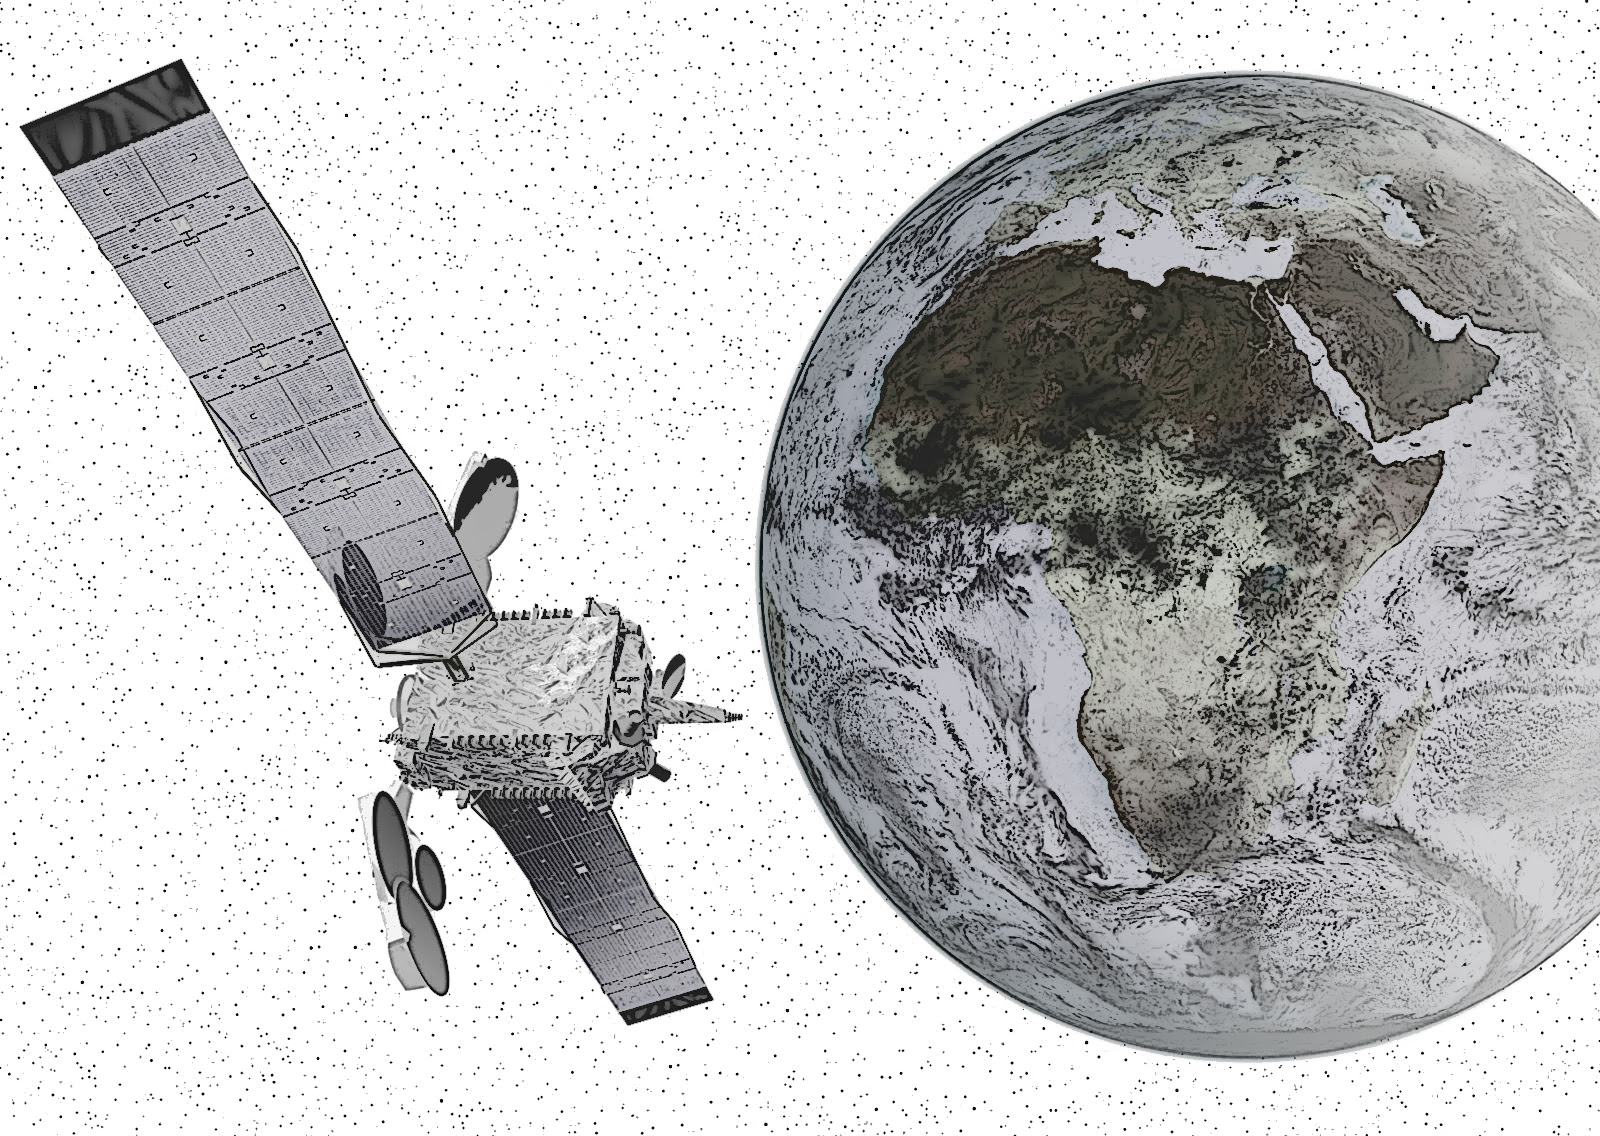
\includegraphics[width=0.93\textwidth]{satelittebis}

                %\vspace{20em}
                %\phantom{.}
            \end{center}
            %\vspace{-1em}
        \end{tabular}
    \end{flushright}

\end{titlepage}
\sloppy
\titlepage


%    \cleardoublepage

    \tableofcontents

%    \cleardoublepage
}

\mainmatter

%-------------------------------------------------------------------------------------------------------------------------------
%-------------------------------------------------------------------------------------------------------------------------------
% Fancy Header Style Options
\pagestyle{fancy}                       % Sets fancy header and footer
\fancyfoot{}                            % Delete current footer settings
%\renewcommand{\chaptermark}[1]{         % Lower Case Chapter marker style
%  \markboth{\chaptername\ \thechapter.\ #1}}{}} %
%\renewcommand{\sectionmark}[1]{         % Lower case Section marker style
%  \markright{\thesection.\ #1}}         %
\fancyhead[LE,RO]{\bfseries\thepage}    % Page number (boldface) in left on even
% pages and right on odd pages
\fancyhead[RE]{\bfseries\nouppercase{\leftmark}}      % Chapter in the right on even pages
\fancyhead[LO]{\bfseries\nouppercase{\rightmark}}     % Section in the left on odd pages
\let\headruleORIG\headrule
\renewcommand{\headrule}{\color{black} \headruleORIG}
\renewcommand{\headrulewidth}{1.0pt}
\arrayrulecolor{black}
\fancypagestyle{plain}{
  \fancyhead{}
  \fancyfoot{}
  \renewcommand{\headrulewidth}{0pt}
}
%-------------------------------------------------------------------------------------------------------------------------------
%-------------------------------------------------------------------------------------------------------------------------------

%\cleardoublepage
\chapter{M\'ethode de tir simple}
\label{chap:tir_simple}
%\minitoc
%---------------------------------------------------------------------------------------------------------
%---------------------------------------------------------------------------------------------------------
\section{Introduction}

Nous allons dans cette partie voir une m\'ethode de r\'esolution num\'erique d'un probl\`eme simple de
contr\^ole optimal utilisant les conditions n\'ecessaires d'optimalit\'e, c'est-\`a-dire le Principe
du Maximum de Pontryagin (PMP), \cf annexe \ref{chap:pmp_fort}. Cette m\'ethode fait partie des m\'ethodes dites indirectes et s'appelle
la m\'ethode de tir simple.
%Vous pouvez consulter la r\'ef\'erence suivante pour une description
%des diff\'erentes m\'ethodes num\'eriques de r\'esolution de probl\`emes de contr\^ole optimal~: A.~V.~Rao,
%\emph{A survey of numerical methods for optimal control}.

%---------------------------------------------------------------------------------------------------------
%---------------------------------------------------------------------------------------------------------
\section{Pr\'esentation de la m\'ethode de tir simple sur un exemple}

\subsection{Le probl\`eme de contr\^ole optimal}

    Consid\'erons le probl\`eme de contr\^ole optimal suivant.
    \leqnomode
    \begin{equation}
    \tagProblem
        \left\{ 
            \begin{array}{l}
                \displaystyle J(u(\cdot))  \coloneqq \displaystyle \frac{1}{2} \int_0^{t_f} u(t)^2 \, \diff t\longrightarrow \min \\[1.0em]
                \dot{x}(t)  =  \displaystyle -x(t)+u(t), \quad  u(t) \in \R, \quad t \in \intervalleff{0}{t_f} \text{ p.p.},\quad x(0) = x_0, \\[1.0em]
                x(t_f) = x_f,
            \end{array}
        \right. 
        \label{eq:ocpSimple}
    \end{equation}
    \reqnomode
    avec $t_f \coloneqq 1$, $x_0 \coloneqq -1$, $x_f \coloneqq 0$ et $\forall\, t \in\intervalleff{0}{t_f}$, $x(t) \in \R$.
    Notons 
    \[
        H(x,p,p^0,u) \coloneqq p \, (-x+u) + p^0\, \frac{1}{2} u^2,
    \]
    le pseudo-hamiltonien associ\'e au probl\`eme \eqref{eq:ocpSimple}.

\subsection{Application du principe du maximum de Pontryagin}

    D'apr\`es le PMP, si $u(\cdot)$ est une solution optimal de \eqref{eq:ocpSimple} (avec $x(\cdot)$ la trajectoire associ\'ee)
    alors il existe un vecteur adjoint $p(\cdot) \in AC(\intervalleff{0}{t_f},\R)$, un scalaire $p^0 \le 0$, tels que $(p(\cdot),p^0) \ne (0,0)$,
    et tels que les \'equations suivantes sont v\'erifi\'ees pour $t\in\intervalleff{0}{t_f}$ p.p. :
    \begin{equation*}
        \left\{ 
            \begin{array}{ll}
                \dot{x}(t)  & = \phantom{-} \partial_p H[t] = -x(t)+u(t),   \\[0.5em]
                \dot{p}(t)  & = -           \partial_x H[t] = p(t),         \\[0.5em]
                0           & = \phantom{-} \partial_u H[t] = p(t)+p^0 u(t),
            \end{array}
        \right. 
    \end{equation*}
    o\`u $[t] := (x(t),p(t),p^0,u(t))$.
    Il n'y a pas d'anormale car si $p^0=0$ alors $p(\cdot)\equiv0$ ce qui est impossible. Ainsi, on a $p^0 < 0$.
%
    Notons 
    $
        u_s(x,p,p^0) \coloneqq - p/p^0,
    $
    la solution de l'\'equation $0 = \partial_u H(x,p,p^0,u)$ pour $(x,p,p^0)$ fix\'e.
    On peut alors fixer arbitrairement $p^0\ne 0$ car pour tout $\alpha \in \Rsp$, $u_s(x,\alpha p, \alpha p^0) = u_s(x,p,p^0)$ et la trajectoire
    associ\'ee reste inchang\'ee. Fixons $p^0 = -1$ et notons maintenant
    \begin{equation*}
        u_s(x,p) = p
        %\label{eq:controleOCPSimple}
    \end{equation*}
    le contr\^ole optimal. De m\^eme, on notera $H(x,p,u)$ le hamiltonien tel que $p^0= -1$.

\subsection{Probl\`eme aux deux bouts}

L'application du PMP nous m\`ene \`a r\'esoudre le \emph{probl\`eme aux deux bouts} (Two Points Boundary Value Problem) suivant~:
    \leqnomode
    \begin{equation}
    \tagProblem
        \left\{ 
            \begin{array}{ll}
                \dot{x}(t)  & = -x(t) + u_s(x(t),p(t)) = -x(t)+p(t),              \\[0.5em]
                \dot{p}(t)  & = \phantom{-}p(t),                                    \\[0.5em]
                x(0)        & = x_0, \quad x(t_f) = x_f.
            \end{array}
        \right. 
        \label{eq:bvpSimple}
    \end{equation}
    \reqnomode
    L'inconnue de ce probl\`eme aux deux bouts est le vecteur adjoint initial $p(0)$.
    En effet si l'on fixe $p_0 \coloneqq p(0)$ alors d'apr\`es le th\'eor\`eme de Cauchy--Lipschitz, il existe une unique solution maximale
    $z(\cdot, x_0, p_0)\coloneqq(x(\cdot, x_0, p_0),p(\cdot, x_0, p_0))$ v\'erifiant la dynamique (sur $x$ et $p$) et la condition initiale
    $z(0, x_0, p_0) = (x_0,p_0)$.
    Le probl\`eme est donc de trouver $p_0$ tel que $x(t_f, x_0, p_0) = x_f$.

\subsection{Fonction de tir et m\'ethode de tir (simple)}

    On va transformer le probl\`eme aux deux bouts \eqref{eq:bvpSimple} en un syt\`eme d'\'equations non lin\'eaires, que l'on appelle \'equations de tir.
    Pour cela, on d\'efinit tout d'abord le syst\`eme hamiltonien 
    \begin{equation*}
        \vv{H}(x,p,u) \coloneqq \left( \frp{H}{p}(x,p,u), -\frp{H}{x}(x,p,u) \right).
        %\label{eq:sysHamTirSimple}
    \end{equation*}
    %
    On note $z \coloneqq (x,p)$, puis $z(\cdot,x_0,p_0)$ la solution de l'\'equation diff\'erentielle $\dot{z}(t) = \vv{H}(z(t), u_s(z(t)))$
    v\'erifiant $z(0,x_0,p_0) = (x_0,p_0)$.
    %
    On d\'efinit enfin la \emph{fonction de tir} suivante :
    \begin{equation}
        \begin{array}{rlll}
            S \colon    & \R    & \longrightarrow   & \R \\
                        & y     & \longmapsto       & S(y) \coloneqq \Pi_x(z(t_f,x_0,y)) - x_f,
        \end{array}
        \label{eq:fonctionDeTirSimple}
    \end{equation}
    o\`u $\Pi_x$ est simplement la projection canonique $\Pi_x(x,p) = x$.
    %
    R\'esoudre le probl\`eme aux deux bouts \eqref{eq:bvpSimple} revient \`a trouver un z\'ero de la fonction de tir, 
    \ie consiste \`a r\'esoudre
    $S(y) = 0.$ C'est ce que l'on appelle 
    la \emph{m\'ethode de tir simple}. On utilise alors une m\'ethode 
    de type Newton pour la r\'esolution, \`a laquelle nous pouvons fournir la jacobienne de $S$.

    \begin{myremark}
        \anoter
        Si $\psol_0$ v\'erifie $S(\psol_0)=0$, alors 
        la courbe int\'egrale $\zsol(\cdot) \coloneqq z(\cdot, x_0, \psol_0)$,
        avec le contr\^ole $\usol(\cdot) \coloneqq u_s(\zsol(\cdot))$,
        est une BC-extr\'emale du probl\`eme \eqref{eq:ocpSimple}, \ie cette extr\'emale satisfait les conditions n\'ecessaires d'optimalit\'e
        donn\'ees par le PMP.
    \end{myremark}

    \begin{myremark}
        \anoter
        La courbe int\'egrale $z(\cdot, z_0)$ est aussi solution du syst\`eme hamiltonien $\dot{z}(t) = \vv{h}(z(t))$, $z(0) = z_0$,
        o\`u $h(z) \coloneqq H(z, u_s(z))$ et $\vv{h} \coloneqq (\partial_p h, -\partial_x h)$.
    \end{myremark}

\subsection{Calcul du z\'ero de la fonction de tir}

    Calculons la solution \`a la main sur cet exemple simple.
    \[
        \dot{p}(t) = p(t) \Longrightarrow p(t) = e^t \, p_0,~ p_0 \coloneqq p(0) \Longrightarrow x(t) = (0.5\, p_0 \,e^{2\,t} + C)\, e^{-t},~ C \in \R.
    \]
    Or $x(0) = x_0$ donc 
    $
        x(t) = (0.5\, p_0 \, (e^{2\,t} - 1) + x_0 )\, e^{-t}
    $
    et finalement, puisque $x_0 = -1$, $x(t_f) = x_f = 0$ et $t_f = 1$, on a
    \[
        \psol_0 = \frac{2 \, (x_f \, e^{t_f} - x_0)}{e^{2\,t_f}-1} = \frac{2}{e^{2}-1} \approx 0.313.
    \]
    La fonction de tir est ici : $p_0 \mapsto (0.5\, p_0 \, (e^{2\,t_f} - 1) + x_0 )\, e^{-t_f} - x_f$.

\section{Pr\'esentation rapide de \hampath}

\subsection{Introduction}

Le code \hampath\ est d\'evelopp\'e par \href{http://caillau.perso.math.cnrs.fr}{J.-B.~Caillau},
\href{http://cots.perso.enseeiht.fr}{O.~Cots} et
\href{http://gergaud.perso.enseeiht.fr}{J.~Gergaud}.
Ce code permet~:
\begin{itemize}
    \item de r\'esoudre les probl\`emes de contr\^ole optimal \`a commandes continues via la m\'ethode du tir simple indirect~;
    \item de r\'esoudre ceux \`a commandes non continues via la m\'ethode du tir multiple indirect~;
    \item de r\'esoudre les familles de probl\`emes de contr\^ole optimal \`a un param\`etre via la m\'ethode homotopique de suivi de chemin
        diff\'erentiel~;
    \item de v\'erifier les conditions du deuxi\`eme ordre via le calcul de points conjugu\'es.
\end{itemize}

\subsection{Sch\'ema g\'en\'eral de \hampath}

L'utilisateur fournit \`a \hampath\ en \fortran\ la fonction de tir $S(y)$ et le hamiltonien maximis\'e $h(z) \coloneqq \max_u H(z,p^0,u)$.
Apr\`es compilation, \hampath\ fournit des fonctions \matlab\ (ou \python)~:
\cmd{hfun}, \cmd{hvfun}, \cmd{exphvfun}, \cmd{dhvfun}, \cmd{expdhvfun}, \cmd{sfun}, \cmd{sjac}, \cmd{ssolve}, \cmd{hampath}\ldots

\begin{myremark}
    La notation \cmd{exphvfun} vient de la notation math\'ematique
    $
        \expmap{z_0}{t_f}{\vv{h}} \coloneqq z(t_f,z_0),
    $
    o\`u $z(\cdot,z_0)$ est la solution de l'edo $\dot{z}(t) = \vv{h}(z(t))$, $z(0) = z_0$.
\end{myremark}

    \begin{figure}[ht!]
        \centering
        \begin{tikzpicture}[scale=0.9]
            \def\widthBox{5.5em}
%            \tikzstyle{rectcoeur}   =[draw,fill=blue!20,text width=\widthBox,minimum height=2em,text centered,rectangle,rounded corners=5pt]
%            \tikzstyle{rectmat}     =[draw,fill=red!20 ,text width=\widthBox,minimum height=2em,text centered,rectangle,rounded corners=5pt]
%            \tikzstyle{rectfor}     =[draw,fill=red!20 ,text width=\widthBox,minimum height=2em,text centered,rectangle,rounded corners=5pt]
            \tikzstyle{rectcoeur}   =[draw=blue!80, thick, fill=white,text width=\widthBox,minimum height=2em,text centered,rectangle,rounded corners=5pt]
            \tikzstyle{rectmat}     =[draw=red!80 , thick, fill=white,text width=\widthBox,minimum height=2em,text centered,rectangle,rounded corners=12pt]
            \tikzstyle{rectfor}     =[draw=red!80 , thick, fill=white,text width=\widthBox,minimum height=2em,text centered,rectangle,rounded corners=12pt]

            \coordinate (O) at (0,0);
            \def\xshift{8em}
            \def\yshift{6em}

            \node[rectmat]      (B1)    at  (                                           O)  {$S(y,\lambda)$};
            \node[rectmat]      (B2)    at  ([xshift= 2.0*\xshift, yshift= 0.0*\yshift] O)  {$h_\lambda(z)$};
            \node[rectcoeur]    (B12)   at  ([xshift=-0.5*\xshift, yshift=-1.0*\yshift] O)  {$\frac{\partial S}{\partial y}(y,\lambda)$};
            \node[rectcoeur]    (B13)   at  ([xshift= 0.5*\xshift, yshift=-1.0*\yshift] O)  {$\frac{\partial S}{\partial \lambda}(y,\lambda)$};
            \node[rectcoeur]    (B14)   at  ([xshift= 0.0*\xshift, yshift=-2.0*\yshift] O)  {$T(r(s))$};
            \node[rectcoeur]    (B15)   at  ([xshift= 0.0*\xshift, yshift=-3.0*\yshift] O)  {\small \cmd{hampath}      \fortran};
            \node[rectcoeur]    (B16)   at  ([xshift=-1.0*\xshift, yshift=-3.0*\yshift] O)  {\small \cmd{ssolve}       \fortran};
            \node[rectcoeur]    (B21)   at  ([xshift= 2.0*\xshift, yshift=-1.0*\yshift] O)  {$\vv{h_\lambda}(z)$};
            \node[rectcoeur]    (B23)   at  ([xshift= 3.0*\xshift, yshift=-2.0*\yshift] O)  {$\diff\vv{h_\lambda}(z)$};
            \node[rectcoeur]    (B22)   at  ([xshift= 2.0*\xshift, yshift=-3.0*\yshift] O)  {\small \cmd{exphvfun}     \fortran}; 
            \node[rectcoeur]    (B24)   at  ([xshift= 3.0*\xshift, yshift=-3.0*\yshift] O)  {\small \cmd{expdhvfun}    \fortran}; 
            \node[rectfor]      (B17)   at  ([xshift=-1.0*\xshift, yshift=-4.0*\yshift] O)  {\small \cmd{ssolve}       \interface};
            \node[rectfor]      (B18)   at  ([xshift= 0.0*\xshift, yshift=-4.0*\yshift] O)  {\small \cmd{hampath}      \interface}; 
            \node[rectfor]      (B25)   at  ([xshift= 2.0*\xshift, yshift=-4.0*\yshift] O)  {\small \cmd{exphvfun}     \interface};
            \node[rectfor]      (B26)   at  ([xshift= 3.0*\xshift, yshift=-4.0*\yshift] O)  {\small \cmd{expdhvfun}    \interface};

            \draw[->,>=latex, densely dashed        ] (B2.west)     -- (                                     B1.east); %hfun vers sfun
            \draw[   >=latex, densely dashed        ] (B22.west)    -| ([xshift= 1.0*\xshift, yshift= 0.0*\yshift] O); %exphvfun vers sfun
            \draw[   >=latex,very thick,color=blue  ] (B1.south)    -- ([xshift= 0.0*\xshift, yshift=-0.5*\yshift] O); %sfun vers un peu plus bas
            \draw[->,>=latex,very thick,color=blue  ] ([xshift= 0.0*\xshift, yshift=-0.5*\yshift] O) -|   (B12.north)  node[gray,near end,left ] {AD};
            \draw[->,>=latex,very thick,color=blue  ] ([xshift= 0.0*\xshift, yshift=-0.5*\yshift] O) -|   (B13.north)  node[gray,near end,right] {AD};
            \draw[->,>=latex,very thick,color=blue  ] (B2.south)    --                                    (B21.north)  node[gray,near end,left ] {AD};
            \draw[->,>=latex,very thick,color=blue  ] (B21.east)    -|                                    (B23.north)  node[gray,midway  ,above] {AD};
            \draw[->,>=latex,very thick,color=blue  ] (B21.south)   --                                    (B22.north)  node[gray,midway  ,left ] {RK};
            \draw[->,>=latex,very thick,color=blue  ] (B23.south)   --                                    (B24.north)  node[gray,midway  ,right] {RK};
            \draw[->,>=latex,very thick,color=blue  ] (B21.south)   |- ([xshift= 3.0*\xshift, yshift=-2.5*\yshift] O);
            \draw[->,>=latex,very thick,color=blue  ] (B1.west)     -|                                    (B16.north)  node[gray,near end,left ] {Newton};
            \draw[   >=latex,very thick,color=blue  ] (B12.west)    -|                                    (B16.north);
            \draw[->,>=latex,very thick,color=blue  ] (B14.south)   --                                    (B15.north)  node[gray,midway  ,left ] {RK +};
            \draw[->,>=latex,very thick,color=blue  ] (B14.south)   --                                    (B15.north)  node[gray,midway  ,right ] {Newton};
            \draw[->,>=latex,very thick,color=blue  ] (B15.south)   --                                    (B18.north);
            \draw[->,>=latex,very thick,color=blue  ] (B16.south)   --                                    (B17.north);
            \draw[->,>=latex,very thick,color=blue  ] (B22.south)   --                                    (B25.north);
            \draw[->,>=latex,very thick,color=blue  ] (B24.south)   --                                    (B26.north);
            \draw[   >=latex,very thick,color=blue  ] (B12.south)   |- ([xshift= 0.0*\xshift, yshift=-1.5*\yshift] O);
            \draw[   >=latex,very thick,color=blue  ] (B13.south)   |- ([xshift= 0.0*\xshift, yshift=-1.5*\yshift] O);
            \draw[   >=latex,very thick,color=blue  ] ([xshift= 0.0*\xshift, yshift=-1.5*\yshift] O) -- (B14.north) node[gray,above,near start,yshift=0.5em]{QR};

            \draw[densely dashed, color=red         ] ([xshift=-1.5*\xshift, yshift=-0.3*\yshift] O) -- ([xshift= 3.5*\xshift, yshift=-0.3*\yshift] O);
            \draw[densely dashed, color=red         ] ([xshift=-1.5*\xshift, yshift=-3.5*\yshift] O) -- ([xshift= 3.5*\xshift, yshift=-3.5*\yshift] O);

            \node[red]  at ([xshift= 1.0*\xshift, yshift= 0.2*\yshift] O) {\fortran\ routines};
            \node[gray] at ([xshift= 3.0*\xshift, yshift=-0.4*\yshift] O) {\fortran\ core};
            \node[red]  at ([xshift= 1.0*\xshift, yshift=-3.7*\yshift] O) {\interface\ routines};
        \end{tikzpicture}
    \caption{
        Sch\'ema g\'en\'eral de \hampath.
        AD signifie Diff\'erentiation Automatique, RK signifie sch\'emas d'int\'egration num\'erique de Runge-Kutta
        utilis\'es pour la r\'esolution d'\'equations diff\'erentielles ordinaires. L'appellation Newton est employ\'ee
        d\`es qu'un solveur d'\'equations non lin\'eaires de type Newton est appel\'e et enfin QR veut dire factorisation QR.
    }
    \label{fig:schema}
    \end{figure}


%---------------------------------------------------------------------------------------------------------
%---------------------------------------------------------------------------------------------------------


%---------------------------------------------------------------------------------------------------------
%---------------------------------------------------------------------------------------------------------
\section{R\'esolution num\'erique}

\begin{myremark} Se rendre dans le r\'epertoire \cmd{TP\_MI} et ex\'ecuter la commande (dans un terminal) :
    \begin{center}
        \cmd{source hampath\_on}
    \end{center}
    Cette commande doit \^etre ex\'ecut\'ee \`a chaque ouverture d'un nouveau terminal.
\end{myremark}

%------------------------------------------------
\subsection{Probl\`eme \eqref{eq:ocpSimple}}

\begin{myExercice} Se rendre dans le r\'epertoire \cmd{TP\_1\_tir\_simple\_pb\_scalaire/exo\_1}.
    \begin{enumerate}
        \item Jeter un \oe il \`a la routine \cmd{control} du fichier \cmd{afun.f90} codant le contr\^ole $u_s(x,p,p^0) = -p/p^0$, $p^0=-1$.
        \item Jeter un \oe il \`a la routine \cmd{hfun} de \cmd{hfun.f90} codant le hamiltonien maximis\'e 
            $h(z) \coloneqq H(z, p^0, u_s(z, p^0))$, $p^0=-1$, $z\coloneqq (x,p)$ et $H(z,p^0,u) = p(-x+u)+p^0 u^2/2$.
        \item Jeter un \oe il \`a la routine \cmd{sfun} de \cmd{sfun.f90} codant la fonction de tir \eqref{eq:fonctionDeTirSimple}.
            On remarquera l'utilisation de la routine \fortran\ \cmd{exphv} pour l'int\'egration num\'erique du syst\`eme hamiltonien.
        \item Compiler le probl\`eme : ex\'ecuter la commande \cmd{hampathCIMI} dans un terminal dans le r\'epertoire de d\'efinition du probl\`eme.
        \item Jeter un \oe il au script \matlab\ \cmd{main11.m} puis l'ex\'ecuter. V\'erifier que l'on retrouve bien $\psol_0 = \frac{2}{e^2-1}$.
    \end{enumerate}
\end{myExercice}

\begin{myremark}
    \anoter
    Les param\`etres du probl\`eme sont transmis via le vecteur \cmd{par}, des fonctions \matlab\ vers les routines \fortran.
\end{myremark}

%------------------------------------------------
\subsection{Ajout de contraintes sur le contr\^ole}

On consid\`ere le probl\`eme de contr\^ole \eqref{eq:ocpSimple} o\`u l'on ajoute la contrainte sur le contr\^ole par
$u(t) \in \intervalleff{-u_\mathrm{max}}{u_\mathrm{max}}$, $u_\mathrm{max}\coloneqq 1$. La condition de maximisation nous donne comme loi de contr\^ole~:
\begin{equation*}
    %\tag{\ref{eq:controleOCPSimple}$^*$}
    u(t) = 
    \left\{
        \begin{array}{ll}
            u_s(x(t),p(t),p^0) = -p(t)/p^0   & \text{ si } \abs{p(t)} \le u_\mathrm{max}, \\[0.5em]
            +u_\mathrm{max}         & \text{ si } p(t) > u_\mathrm{max}, \\[0.5em]
            -u_\mathrm{max}         & \text{ si } p(t) < -u_\mathrm{max}.
        \end{array}
    \right.
    %\label{eq:controleOCPSimpleContraint}
\end{equation*}

\begin{myExercice} Se rendre dans le r\'epertoire \cmd{TP\_1\_tir\_simple\_pb\_scalaire/exo\_2\_contraintes\_sur\_u}.
    \begin{enumerate}
        \item D\'ecommenter la partie codant pour l'ajout de la contrainte sur le contr\^ole dans le fichier \cmd{afun.f90}.
            Attention, $u_\mathrm{max}$ est donn\'e dans le vecteur \cmd{par}.
        \item Compiler le probl\`eme.
        \item Jeter un \oe il au script \matlab\ \cmd{main12.m} puis l'ex\'ecuter.
    \end{enumerate}
\end{myExercice}



%
%\cleardoublepage
\chapter{Tir simple versus tir multiple}
\label{chap:tir_simple_vs_multiple}
%\minitoc
%---------------------------------------------------------------------------------------------------------
%---------------------------------------------------------------------------------------------------------
\section{Double int\'egrateur : \'energie min}

Consid\'erons le probl\`eme de contr\^ole optimal suivant :
\leqnomode
\begin{equation*}
\tagProblem
    \left\{ 
        \begin{array}{l}
            \displaystyle J(u(\cdot)) \coloneqq \displaystyle \frac{1}{2} \int_0^{t_f} u(t)^2 \, \diff t\longrightarrow \min            \\[1.0em]
            \dot{x}_1(t)    =  \displaystyle x_2(t)                                                                                     \\[0.5em]
            \dot{x}_2(t)    =  \displaystyle u(t), \quad \abs{u(t)} \le u_\mathrm{max}, \quad t \in \intervalleff{0}{t_f} \text{ p.p.}, \\[1.0em]
            x(0) = x_0 , \quad x(t_f) = x_f,
        \end{array}
    \right. 
    \label{eq:ocp_DI_min_E}
\end{equation*}
\reqnomode
avec $t_f \coloneqq 1$, $x_0 \coloneqq (-1,0)$, $x_f \coloneqq (0,0)$ et $\forall\, t \in\intervalleff{0}{t_f}$, $x(t) = (x_1(t), x_2(t)) \in \R^2$.
Notons 
\[
    H(x,p,p^0,u) \coloneqq p_1\, x_2 + p_2\, u + p^0\, \frac{1}{2} u^2, \quad x = (x_1, x_2), \quad p = (p_1, p_2),
\]
le pseudo-hamiltonien. On consid\`ere le cas normal et on fixe $p^0 = -1$. La condition de maximisation
nous donne comme loi de contr\^ole~:
\begin{equation*}
    u(t) = 
    \left\{
        \begin{array}{ll}
            u_s(x(t),p(t)) \coloneqq p_2(t)   & \text{ si } \abs{p_2(t)} \le u_\mathrm{max}, \\[0.5em]
            +u_\mathrm{max}                      & \text{ si } p_2(t) > u_\mathrm{max}, \\[0.5em]
            -u_\mathrm{max}                      & \text{ si } p_2(t) < -u_\mathrm{max}.
        \end{array}
    \right.
\end{equation*}
%
La fonction de tir est donn\'ee par :
\begin{equation*}
    \begin{array}{rlll}
        S \colon    & \R^2    & \longrightarrow   & \R^2 \\
                    & y       & \longmapsto       & S(y) \coloneqq x(t_f,x_0,y) - x_f,
    \end{array}
\end{equation*}
o\`u $y$ joue ici le r\^ole du vecteur adjoint initial $p(0)$.

\begin{myExercice} Se rendre dans le r\'epertoire \cmd{TP\_2\_tir\_simple\_et\_multiple\_double\_integrateur/exo\_1\_energie\_min}.
    \begin{enumerate}
        \item Compl\'eter \cmd{control}, \cmd{hfun} et \cmd{sfun}, respectivement dans les fichiers \cmd{afun.f90}, \cmd{hfun.f90} et \cmd{sfun.f90}.
            Attention pour \cmd{sfun}, m\^eme si $x_f = (0,0)$, il est pass\'e en param\`etre \`a l'aide du vecteur \cmd{par} : $x_f = par(5:6)$.
        \item Compiler le probl\`eme.
        \item Jeter un \oe il au script \matlab\ \cmd{main21.m} puis l'ex\'ecuter. Vous pouvez tester la r\'esolution du probl\`eme pour deux valeurs de
            $u_\mathrm{max}$.
    \end{enumerate}
\end{myExercice}

\begin{myremark}
    \anoter
    La loi de commande $\usol(\cdot)$ associ\'ee \`a la solution des \'equations de tir est lisse lorsque $u_\mathrm{max} \ge 6$.
    Pour $u_\mathrm{max} < 6$, la loi de commande perd en r\'egularit\'e. Pour $u_\mathrm{max} = 4.5$, elle est continue mais pas $C^1$,
    seulement $C^1$ par morceaux (elle est m\^eme lisse par morceaux).
\end{myremark}

%---------------------------------------------------------------------------------------------------------
%---------------------------------------------------------------------------------------------------------
\section{Double int\'egrateur : temps min}

Consid\'erons le probl\`eme \eqref{eq:ocp_DI_min_E} o\`u l'on remplace le crit\`ere par le suivant : $J(u(\cdot), t_f) \coloneqq t_f$.
On remarque alors que dans ce cas, le temps final $t_f$ est libre. Fixons de plus la borne sur le contr\^ole : $u_\mathrm{max} = 1$.
%
Notons le pseudo-hamiltonien
\[
    H(x,p,u) \coloneqq p_1\, x_2 + p_2\, u.
\]
La condition de maximisation nous donne comme loi de contr\^ole~:
\begin{equation*}
    u(t) = 
    \left\{
        \begin{array}{ll}
            +u_\mathrm{max}  & \text{ si } p_2(t) > 0, \\[0.5em]
            -u_\mathrm{max}  & \text{ si } p_2(t) < 0, \\[0.5em]
            ?                & \text{ si } p_2(t) = 0.
        \end{array}
    \right.
\end{equation*}

\begin{myremark}
    \anoter
    Il n'est pas possible d'avoir $p_2(t) = 0$ sur un intervalle de temps non r\'eduit \`a un point. Ainsi, nous pouvons ignorer ce cas.
\end{myremark}

Puisque $t_f$ est libre, le PMP nous donne la condition de transversalit\'e \[H(x(t_f), p(t_f), u(t_f)) = -p^0, \]
o\`u l'on fixe toujours $p^0=-1$ car nous ne consid\'erons que le cas normal. 
%

%-----------------------------------------------------
\subsection{Tir simple}

La fonction de tir simple est donn\'ee par~:
\begin{equation*}
    \begin{array}{rlll}
        S \colon    & \R^3      & \longrightarrow   & \R^3 \\
        & y\coloneqq(p_0, t_f)  & \longmapsto       & S(y) \coloneqq
        \begin{bmatrix}
            x(t_f,x_0,p_0) - x_f \\
            H(x(t_f,x_0,p_0),p(t_f,x_0,p_0),u(t_f))+p^0
        \end{bmatrix}.
    \end{array}
\end{equation*}

\begin{myExercice} Se rendre dans le r\'epertoire \cmd{TP\_2\_tir\_simple\_et\_multiple\_double\_integrateur/} \cmd{exo\_2\_temps\_min\_tir\_simple}.
    \begin{enumerate}
        \item Compl\'eter \cmd{control}, \cmd{hfun} et \cmd{sfun}, respectivement dans les fichiers \cmd{afun.f90}, \cmd{hfun.f90} et \cmd{sfun.f90}.
            Attention pour \cmd{sfun}, m\^eme si $x_f = (0,0)$, il est pass\'e en param\`etre \`a l'aide du vecteur \cmd{par} : $x_f = par(3:4)$.
        \item Compiler le probl\`eme.
        \item Jeter un \oe il au script \matlab\ \cmd{main22.m} puis l'ex\'ecuter.
    \end{enumerate}
\end{myExercice}

\begin{myremark}
    \anoter
    Remarquer que le solveur \cmd{fsolve} de \matlab\ ne fait qu'une it\'eration mais ne progresse pas.
\end{myremark}

%-----------------------------------------------------
\subsection{Tir multiple}

Nous introduisons quelques notations pour clarifier l'expression de la fonction de tir multiple que l'on d\'efinit ci-apr\`es.
On note $H_+(z) \coloneqq H(z, u_\mathrm{max})$, $H_-(z) \coloneqq H(z, -u_\mathrm{max})$ et $\vv{H_+}$, $\vv{H_-}$ les syst\`emes hamiltoniens associ\'es.
Pour d\'efinir la fonction de tir multiple, nous devons n\'ecessairement conna\^itre la structure du contr\^ole. Ici, nous savons que la structure 
contient deux arcs : $+u_\mathrm{max}$ suivi de $-u_\mathrm{max}$. Le PMP nous donne qu'\`a l'instant de la commutation (not\'e $t_1$), on a $p_2(t_1) = 0$.
Nous pouvons maintenant d\'efinir la fonction de tir multiple (de structure), qui est donn\'ee par~:
\begin{equation*}
    \begin{array}{rlll}
        S \colon    & \R^4          & \longrightarrow   & \R^4 \\
        & y\coloneqq(p_0, t_f, t_1) & \longmapsto       & S(y) \coloneqq
        \begin{bmatrix}
            \Pi_x\left( z_f \right) - x_f \\[0.5em]
            H_-(z_f)+p^0                  \\[0.5em]
            \Pi_{p_2}\left( z_1 \right)
        \end{bmatrix},
    \end{array}
\end{equation*}
o\`u
\[
    z_1 \coloneqq \expmap{x_0,p_0}{t_1}{\vv{H_+}}, \quad z_f \coloneqq \expmap{z_1}{(t_f-t_1)}{\vv{H_-}}.
\]
On rappelle que $\Pi_x(z) = x$ avec $z=(x,p)$, $p=(p_1, p_2)$, et on d\'efinit $\Pi_{p_2}(z) = p_2$.

\begin{myExercice} Se rendre dans le r\'epertoire \cmd{TP\_2\_tir\_simple\_et\_multiple\_double\_integrateur/}
    \cmd{exo\_3\_temps\_min\_tir\_multiple\_de\_structure}.
    \begin{enumerate}
        \item Jeter un \oe il \`a la routine \cmd{control} de \cmd{afun.f90}. Noter l'utilisation de la variable \cmd{iarc} indiquant si l'on se trouve
            sur le premier o\`u le second arc.
        \item Jeter un \oe il \`a la routine \cmd{hfun} de \cmd{hfun.f90}. Elle reste inchang\'ee.
        \item Compl\'eter \cmd{sfun} de \cmd{sfun.f90}. Attention \`a bien utiliser la variable \cmd{iarc}.
        \item Compiler le probl\`eme.
        \item Jeter un \oe il au script \matlab\ \cmd{main23.m} puis l'ex\'ecuter.
    \end{enumerate}
\end{myExercice}

\begin{myremark}
    \anoter
    Comparer la pr\'ecision de la solution num\'erique entre le tir multiple et le tir simple. On notera que pour le tir multiple, nous avons
    besoin d'une information suppl\'ementaire : la structure du contr\^ole optimal.
\end{myremark}


%\cleardoublepage
\chapter{M\'ethode homotopique, r\'egularisation et tir multiple}
\label{chap:homotopie}
%\minitoc
Consid\'erons le probl\`eme de contr\^ole optimal suivant (double int\'egrateur, minimisation $L^1$) :
\leqnomode
\begin{equation*}
\tagProblem
    \left\{ 
        \begin{array}{l}
            \displaystyle J(u(\cdot)) \coloneqq \displaystyle \int_0^{t_f} \abs{u(t)} \, \diff t\longrightarrow \min            \\[1.0em]
            \dot{x}_1(t)    =  \displaystyle x_2(t)                                                                                     \\[0.5em]
            \dot{x}_2(t)    =  \displaystyle u(t), \quad \abs{u(t)} \le u_\mathrm{max}, \quad t \in \intervalleff{0}{t_f} \text{ p.p.}, \\[1.0em]
            x(0) = x_0 , \quad x(t_f) = x_f,
        \end{array}
    \right. 
    \label{eq:ocp_DI_min_L1}
\end{equation*}
\reqnomode
avec $t_f \coloneqq 3$, $x_0 \coloneqq (-1,0)$, $x_f \coloneqq (0,0)$ et $\forall\, t \in\intervalleff{0}{t_f}$, $x(t) = (x_1(t), x_2(t)) \in \R^2$.
%
Notons 
\[
    H(x,p,p^0,u) \coloneqq p_1\, x_2 + p_2\, u + p^0\, \abs{u}, \quad x = (x_1, x_2), \quad p = (p_1, p_2),
\]
le pseudo-hamiltonien. On consid\`ere le cas normal et on fixe $p^0 = -1$. La condition de maximisation
nous donne comme loi de contr\^ole~:
\begin{equation*}
    u(t) = 
    \left\{
        \begin{array}{ll}
            \sign(p_2(t))\, u_\mathrm{max}      & \text{ si } \abs{p_2(t)}+p^0 > 0, \\[0.5em]
            0                   & \text{ si } \abs{p_2(t)}+p^0 < 0, \\[0.5em]
            ?                   & \text{ si } \abs{p_2(t)}+p^0 = 0.
        \end{array}
    \right.
\end{equation*}
%

Nous voulons ici r\'esoudre le probl\`eme par une m\'ethode de tir multiple. Nous avons donc besoin dans un premier temps, 
de d\'eterminer la structure du contr\^ole. Pour ce faire, nous pourrions utiliser un m\'ethode de tir simple en prenant certaines
pr\'ecautions, notamment sur le calcul de la jacobienne de la fonction de tir. Une autre possibilit\'e est d'utiliser une
m\'ethode homotopique diff\'erentielle de suivi de chemin combin\'ee \`a une m\'ethode de r\'egularisation.
%
Nous introduisons donc le crit\`ere suivant afin de r\'egulariser le contr\^ole optimal : 
\begin{equation}
    J_\lambda(u(\cdot)) \coloneqq \displaystyle \int_0^{t_f} \abs{u(t)}^{2-\lambda} \, \diff t, \quad \lambda \in \intervallefo{0}{1}.
    \label{eq:critere_regularisant}
\end{equation}

%---------------------------------------------------------------------------------------------------------
%---------------------------------------------------------------------------------------------------------
\section{R\'esolution du probl\`eme r\'egularis\'e}

Nous consid\'erons ici le probl\`eme \eqref{eq:ocp_DI_min_L1} o\`u l'on remplace le crit\`ere $J$ par $J_\lambda$ d\'efinit
en \eqref{eq:critere_regularisant}. Le pseudo-hamiltonien est donn\'e par :
\[
    H_\lambda(x,p,p^0,u) \coloneqq p_1\, x_2 + p_2\, u + p^0\, \abs{u}^{2-\lambda}
\]
et le contr\^ole maximisant s'\'ecrit
\[
    u(t) = \sign(p_2(t))\, \left( - \frac{\abs{p_2(t)}}{p^0\, (2-\lambda)} \right)^{\frac{1}{1-\lambda}}.
\]
La fonction de tir est simplement donn\'ee par :
\begin{equation*}
    \begin{array}{rlll}
        S \colon    & \R^2    & \longrightarrow   & \R^2 \\
                    & y       & \longmapsto       & S(y) \coloneqq x(t_f,x_0,y) - x_f.
    \end{array}
\end{equation*}

\begin{myExercice} Se rendre dans le r\'epertoire \cmd{TP3\_homotopie\_regularisation\_double\_integrateur/}\cmd{exo\_1\_regularisation}.
    \begin{enumerate}
        \item Compl\'eter seulement \cmd{hfun} dans \cmd{hfun.f90}.
        \item Compiler le probl\`eme.
        \item Jeter un \oe il au script \matlab\ \cmd{main31.m} puis l'ex\'ecuter.
    \end{enumerate}
\end{myExercice}

%---------------------------------------------------------------------------------------------------------
%---------------------------------------------------------------------------------------------------------
\section{R\'esolution du probl\`eme de minimisation $L^1$}

D'apr\`es la r\'egularisation (pour $\lambda$ proche de 1), le contr\^ole optimal solution du probl\`eme \eqref{eq:ocp_DI_min_L1}
poss\`ede trois arcs : $u=u_\mathrm{max}$ suivi de $u=0$ puis $u=-u_\mathrm{max}$.
On note $H_+(z) \coloneqq H(z, p^0, u_\mathrm{max})$, $H_-(z) \coloneqq H(z, p^0, -u_\mathrm{max})$, $H_0(z) \coloneqq H(z, p^0, 0)$
et $\vv{H_+}$, $\vv{H_-}$, $\vv{H_0}$ les syst\`emes hamiltoniens associ\'es.
La fonction de tir correspondant \`a cette structure s'\'ecrit :
\begin{equation*}
    \begin{array}{rlll}
        S \colon    & \R^4          & \longrightarrow   & \R^4 \\
        & y\coloneqq(p_0, t_1, t_2) & \longmapsto       & S(y) \coloneqq
        \begin{bmatrix}
            \Pi_{p_2}\left( z_1 \right) + p^0   \\[0.5em]
            \Pi_{p_2}\left( z_2 \right) - p^0   \\[0.5em]
            \Pi_x\left( z_f \right) - x_f
        \end{bmatrix},
    \end{array}
\end{equation*}
o\`u
\[
    z_1 \coloneqq \expmap{x_0,p_0}{t_1}{\vv{H_+}}, \quad z_2 \coloneqq \expmap{z_1}{(t_2-t_1)}{\vv{H_0}},
    \quad z_f \coloneqq \expmap{z_2}{(t_f-t_2)}{\vv{H_-}}.
\]

\begin{myExercice} Se rendre dans le r\'epertoire \cmd{TP3\_homotopie\_regularisation\_double\_integrateur/}\cmd{exo\_2\_min\_L1}.
    \begin{enumerate}
        \item Compl\'eter \cmd{control}, \cmd{hfun} et \cmd{sfun}, respectivement dans les fichiers \cmd{afun.f90}, \cmd{hfun.f90} et \cmd{sfun.f90}.
        \item Compiler le probl\`eme.
        \item Compl\'eter le script \matlab\ \cmd{main32.m} puis l'ex\'ecuter. Il faut fournir au solveur des \'equations de tir, la pr\'ediction
            initiale du vecteur adjoint initial $p_0$ et des instants de commutations $t_1$ et $t_2$. Utiliser pour cela, la solution du probl\`eme 
            r\'egularis\'e avec $\lambda$ proche de $1$.
    \end{enumerate}
\end{myExercice}


%\cleardoublepage
\chapter{Transfert orbital}
\label{chap:transfert_orbital}
%\minitoc
\section{Introduction}

Le syst\`{e}me consid\'{e}r\'{e} est un satellite de masse fix\'{e} $m$ lib\'{e}r\'{e}
par une fus\'{e}e dans le plan de l'\'{e}quateur; l'orbite initiale du satellite est
une ellipse de forte excentricit\'{e}, voir figure~\ref{figtransfert}. L'objectif de ce travail est de r\'{e}aliser
le transfert en temps minimal de cette orbite elliptique \`{a} une orbite circulaire 
g\'{e}ostationnaire. 

\begin{figure}[ht!]
\centering
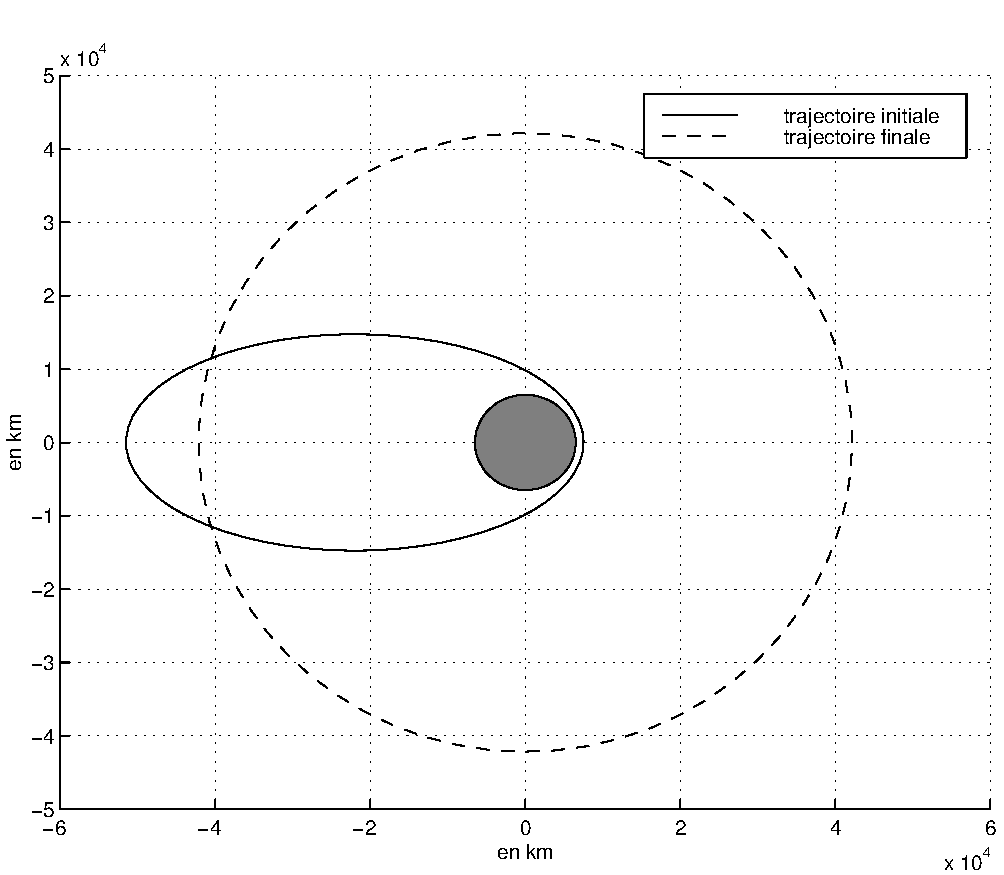
\includegraphics[height=5.0cm]{./fig1transfert}
\caption{\label{figtransfert}Transfert orbital 2D.}
\end{figure}

\section{R\'esolution du probl\`eme en temps minimal}

Consid\'erons le probl\`eme de transfert orbital \`a temps minimal suivant~:
\leqnomode
\begin{equation}\label{eq:transfert_temps_min}
    \tagProblem
        \left\{
            \begin{array}{l}
                \displaystyle J(u(\cdot), t_f) = t_f \longrightarrow \min                                \\[1.0em]
                \displaystyle \dot{x}_1(t) = x_3(t), \\[0.5em]
                \displaystyle \dot{x}_2(t) = x_4(t), \\[0.5em]
                \displaystyle \dot{x}_3(t) = -\frac{\mu\, x_1(t)}{{r(t)}^3} + u_1(t), \\[0.5em]
                \displaystyle \dot{x}_4(t) = -\frac{\mu\, x_2(t)}{{r(t)}^3} + u_2(t),
                \quad \norme{u(t)} \le \gamma_\mathrm{max}, 
                \quad t \in \intervalleff{0}{t_f} \text{ p.p.}, \quad u(t) \coloneqq(u_1(t),u_2(t)),     \\[1.0em]
                \displaystyle x_1(0) = x_{0,1},   \quad x_2(0) = x_{0,2},  \quad x_3(0) = x_{0,3}, \quad x_4(0) = x_{0,4},  \\[1.0em]
                \displaystyle r(t_f)^2 = r_f^2, \quad
                \displaystyle x_3(t_f) = - \sqrt{\frac{\mu}{r_f^3}}\, x_2(t_f), \quad
                \displaystyle x_4(t_f) = \sqrt{\frac{\mu}{r_f^3}}\, x_1(t_f),
            \end{array} 
        \right.
\end{equation}
\reqnomode
avec $r(t) \coloneqq \sqrt{x_1(t)^2 + x_2(t)^2}$. Les unit\'es choisies sont le kilom\`etre pour les distances et l'heure pour les temps, \cf
table \ref{table:transfert_temps_min_data}.

\begin{table}[ht!]
    \centering
    \begin{tabular}{lll}
        \medhrule
        Param\`etre                                & Valeur & Unit\'e   \\
        \bighrule
        $\mu$                   & $5.1658620912\times10^{12}$  & km$^3$ h$^{-2}$ \\
        $r_f$                   & $42165$                           & km \\
        $\gamma_\mathrm{max}$   & $388.8$                           & km h$^{-2}$ \\
        \medhrule
        \\
    \end{tabular}
    \caption{Unit\'e et valeurs des param\`etres constants. Cette valeur de $\gamma_\mathrm{max}$ correspond \`a une acc\'el\'eration de 60N et \`a
    une masse de 2000kg, \cf $\gamma_\mathrm{max} = \frac{F_\mathrm{max}}{m} = \frac{60 \times 3600^2}{2000 \times 10^3} = 388.8$.}
    \label{table:transfert_temps_min_data}
\end{table}

Le pseudo-hamiltonien est donn\'e par : 
\[
    H(x,p,u) = x_3\, p_1 + x_4\, p_2 + \left(u_1 - \frac{\mu\, x_1}{\norme{r}^3}\right) p_3 + \left(u_2 - \frac{\mu\, x_2}{\norme{r}^3}\right) p_4.
\]
On consid\`ere le cas normal et on fixe $p^0=-1$.
La condition de maximisation nous donne comme loi de commande :
\[
    u(t) = \usol(z(t)) \coloneqq \frac{\gamma_\mathrm{max}}{\sqrt{p_3(t)^2+p_4(t)^2}} \left( p_3(t) , p_4(t) \right).
\]
Le temps final \'etant libre, on a la condition au temps final $H(x(t_f), p(t_f), u(t_f)) = -p^0$ et
puisque le point terminal sur l'orbite final n'est pas enti\`erement fix\'e, le PMP nous donne la condition de transversalit\'e en $t_f$ 
suivante :
\[
    x_2(t_f) \left( p_1(t_f) + \sqrt{\frac{\mu}{r_f^3}}\, p_4(t_f) \right) = x_1(t_f) \left( p_2(t_f) - \sqrt{\frac{\mu}{r_f^3}}\, p_3(t_f) \right).
\]
En introduisant $\alpha \coloneqq \sqrt{\frac{\mu}{r_f^3}}$, la fonction de tir multiple s'\'ecrit :
\begin{equation*}
    \begin{array}{rlll}
        S \colon    & \R^5          & \longrightarrow   & \R^5 \\
        & (p_0, t_f)      & \longmapsto       &
        \begin{bmatrix}
            \sqrt{x_1(t_f, z_0)^2 + x_2(t_f, z_0)^2} - r_f \\[0.5em]
            x_3(t_f, z_0) + \alpha\, x_2(t_f, z_0) \\[0.5em]
            x_4(t_f, z_0) - \alpha\, x_1(t_f, z_0) \\[0.5em]
            x_2(t_f, z_0) \left( p_1(t_f, z_0) + \alpha\, p_4(t_f, z_0) \right) - x_1(t_f, z_0) \left( p_2(t_f, z_0) - \alpha\, p_3(t_f, z_0) \right) \\[0.5em]
            H(z(t_f, z_0), \usol(z(t_f, z_0))) + p^0
        \end{bmatrix},
    \end{array}
\end{equation*}
o\`u $z_0 \coloneqq (x_0, p_0)$, $x_0 \coloneqq (x_{0,1}, x_{0,2}, x_{0,3}, x_{0,4})$, $z(\cdot, z_0) \coloneqq (x(\cdot, z_0), p(\cdot, z_0))$ et
$x \coloneqq (x_1, x_2, x_3, x_4)$, $p\coloneqq (p_1, p_2, p_3, p_4)$.

\begin{myremark}
    Pour la r\'esolution num\'erique, il est pr\'ef\'erable de remplacer l'\'equation $r(t_f)^2 = r_f^2$ par $r(t_f) = r_f$.
\end{myremark}

\begin{myExercice} Se rendre dans le r\'epertoire \cmd{TP4\_transfert\_orbital\_temps\_min}.
    \begin{enumerate}
        \item Compl\'eter seulement \cmd{sfun} dans \cmd{sfun.f90}.
        \item Compiler le probl\`eme.
        \item Jeter un \oe il au script \matlab\ \cmd{main41.m} puis l'ex\'ecuter.
    \end{enumerate}
\end{myExercice}






\makeatletter
\renewcommand{\@chapapp}{\textsc{Annexe}}
\makeatother

\begin{appendix}

\chapter{(Annexe) Principe du Maximum de Pontryagin (PMP)}
\label{chap:pmp_fort}
Dans ce chapitre nous pr\'esentons le \emph{principe du maximum de Pontryagin} :
\begin{quotation}
\newblock L.~S. Pontryagin, V.~G. Boltyanski{\u\i}, R.~V. Gamkrelidze \& E.~F. Mishchenko,
\newblock \emph{The Mathematical Theory of Optimal Processes},
\newblock Translated from the Russian by K. N. Trirogoff, edited by L. W. Neustadt, Interscience Publishers John Wiley \& Sons, Inc., New York-London, 1962.
\end{quotation}
Pour un probl\`eme de contr\^ole optimal donn\'e, ce principe nous fournit des conditions n\'ecessaires d'optimalit\'e
que doit v\'erifier toute solution de ce probl\`eme.

%-----------------------------------------------------------------------------------------------------------------------------------------------
%-----------------------------------------------------------------------------------------------------------------------------------------------
\section{Formulation du probl\`eme de contr\^ole optimal}

Consid\'erons le probl\`eme de contr\^ole optimal suivant~:
\leqnomode
\begin{equation}
\tag{$\mathrm{OCP}$}
    \left\{ 
        \begin{array}{l}
            \displaystyle J(x_0,u(\cdot),t_0,t_f)   \coloneqq   \displaystyle g(t_0, x_0, t_f, x(t_f)) +
                                                \int_{t_0}^{t_f} f^0(t,x(t),u(t)) \, \diff t\longrightarrow \min \\[1.0em]
            \dot{x}(t)                      =   \displaystyle f(t,x(t),u(t)), 
                                                \quad  u(t) \in \U, 
                                                \quad t \in \intervalleff{t_0}{t_f} \text{ p.p.},
                                                \quad x(t_0) = x_0, \\[1.0em]
            c(t_0,x_0,t_f,x(t_f)) = 0,
        \end{array}
    \right. 
\label{eq:ocpGeneral}
\end{equation}
\reqnomode

C'est un probl\`eme tr\`es g\'en\'eral sous la forme de Bolza avec une dynamique non autonome, 
dont les instants initial et final sont libres, o\`u l'on consid\`ere des conditions aux limites m\'elang\'ees
et o\`u le contr\^ole peut \'eventuellement \^etre contraint. On d\'efinit les hypoth\`eses suivantes.

\begin{myassumption}
    \label{hyp:pmp}
    Consid\'erons une EDO contr\^ol\'ee non autonome $\dot{x}(t) = f(t,x(t),u(t)),$ o\`u $f$ est une application de classe
    $\xCn{1}$ de $\I \times \Omega \times \U$ dans $\R^n$, $\I$ un intervalle ouvert de $\R$, $\Omega$ un ouvert de $\R^n$
    et $\U$ un ensemble \empha{quelconque} de $\R^m$. Consid\'erons de plus une fonction $f^0$ de classe
    $\xCn{1}$ sur $\I \times \Omega \times \U$ et deux applications\footnotemark\ $g$ et $c$ de classe $\xCn{1}$ de
    $\I \times \Omega \times \I \times \Omega$ respectivement sur $\R$ et $\R^p$, $p \le 2(n+1)$.
    Notons $$X_c \coloneqq \enstq{(t_0,x_0,t_f,x_f) \in \I \times \Omega \times \I \times \Omega}{c(t_0,x_0,t_f,x_f) = 0}$$
    et supposons que $c'(t_0,x_0,t_f,x_f)$ est surjective pour tout
    $(t_0,x_0,t_f,x_f) \in X_c$.
\end{myassumption}
\footnotetext{On notera $(t_0, x_0, t_f, x_f)$ l'argument des applications $g$ et $c$. On \'ecrira donc $\frp{g}{x_f}$ la d\'eriv\'ee
        partielle de $g$ par rapport \`a la quatri\`eme variable.}

\begin{myremark}
    On peut supposer seulement que $f$ et $f^0$ sont $\xCn{0}$ par rapport \`a $t$ et $u$.
\end{myremark}

%\pagebreak

%
On cherche alors une solution $(x_0,u(\cdot),t_0,t_f)$, $x_0 \in \Omega$, $u(\cdot) \in L^\infty(\intervalleff{t_0}{t_f},\U)$, 
$0 \le t_0 \le t_f$ dans $\R$, telle que la trajectoire associ\'ee \empha{$\mathbf{t \mapsto x(t) \coloneqq x(t,t_0,x_0,u(\cdot))}$} soit d\'efinie sur 
$\intervalleff{t_0}{t_f}$ et telle que la contrainte diff\'erentielle, la contrainte sur le contr\^ole et les conditions
aux limites soient v\'erifi\'ees, et qui de plus minimise le crit\`ere.


%-------------------------------------------------------------------------------------------------------------------------
%-------------------------------------------------------------------------------------------------------------------------
\section{Principe du Maximum de Pontryagin}

\'Enon\c cons maintenant le Principe du Maximum de Pontryagin (PMP).

\envbox[theorem][Principe du Maximum de Pontryagin]{
    Si $(x_0,u(\cdot),t_0,t_f)$, avec $x(\cdot)$ la trajectoire associ\'ee, est solution du probl\`eme \eqref{eq:ocpGeneral} 
    sous les hypoth\`eses \ref{hyp:pmp},
    alors il existe un \emph{vecteur adjoint} $p(\cdot) \in AC(\intervalleff{t_0}{t_f},(\R^n)^*)$, un r\'eel $p^0\le 0$,
    tels que \emphb{$(p(\cdot),p^0)\ne(0,0)$}, et un multiplicateur \emphb{$\lambda \in (\R^p)^*$}, 
    tels que les \'equations suivantes sont v\'erifi\'ees pour $t\in\intervalleff{t_0}{t_f}$ p.p.~:
    \begin{equation}
        \label{eq:pmp_equations_hamilton}
        \begin{aligned}
            \dot{x}(t)              &= \phantom{-}\frp{H}{p}(t,x(t),p(t),p^0,u(t)), \\
            \dot{p}(t)              &=           -\frp{H}{x}(t,x(t),p(t),p^0,u(t)),
        \end{aligned}
    \end{equation}
    o\`u $
            H(t,x,p,p^0,u) \coloneqq p\, f(t,x,u) + p^0 \, f^0(t,x,u)
        $
    est le pseudo-hamiltonien associ\'e au probl\`eme \eqref{eq:ocpGeneral},
    et on a la condition de maximisation du hamiltonien suivante pour $t\in\intervalleff{t_0}{t_f}$ p.p.~:
    \begin{equation}
        \label{eq:pmp_condition_maximisation}
            H(t,x(t),p(t),p^0,u(t)) = \max_{\footnotesize w\in\U} H(t,x(t),p(t),p^0,w).
    \end{equation}
    Les conditions aux limites $c(t_0,x_0,t_f,x(t_f)) = 0$ et $x(t_0)=x_0$ sont v\'erifi\'ees et on a en plus les conditions de transversalit\'e suivantes~:
    \begin{equation}
        p(t_0) = - \left( \lambda \, \frp{c}{x_0} + p^0 \, \frp{g}{x_0} \right), \quad
        p(t_f) = \left( \lambda \, \frp{c}{x_f} + p^0 \, \frp{g}{x_f} \right),
        \label{eq:pmp_conditions_transversalite}
    \end{equation}
    appliqu\'e en $(t_0,x_0,t_f,x(t_f))$.
    %
    Enfin, puisque les temps initial et final sont libres, si $u(\cdot)$ est continu aux temps $t_0$, respectivement $t_f$, alors on a
    les conditions sur le hamiltonien suivantes~:
    \begin{equation}
        H[t_0] = \left( \lambda \, \frp{c}{t_0} + p^0 \, \frp{g}{t_0} \right), \quad
        H[t_f] = - \left( \lambda \, \frp{c}{t_f} + p^0 \, \frp{g}{t_f} \right),
%        H(x(t_f),p(t_f),p^0,u(t_f)) = - \left( \sum_{i=1}^{p} \mu_i \, \frp{c_i}{t}(t_f,x(t_f)) + p^0 \, \frac{\partial g}{\partial t}(t_f,x(t_f)) \right).
        \label{eq:pmp_conditions_hamiltonien}
    \end{equation}
    toujours appliqu\'e en $(t_0,x_0,t_f,x(t_f))$ et o\`u $[t] \coloneqq (t,x(t),p(t),p^0,u(t))$.
    \label{thm:pmp_fort_general}
}

\begin{myremark}
    On rappelle~:
    $\displaystyle \lambda \frp{c}{x_0} = \sum_{i=1}^{p} \lambda_i \, \frp{c_i}{x_0},$ avec $\lambda \coloneqq (\lambda_1, \cdots, \lambda_p)$.
\end{myremark}

\begin{myremark}
    La convention $p^0\le 0$ conduit au principe du \emph{maximum} tandis que $p^0 \ge 0$ conduit au principe du \emph{minimum}, \ie 
    la condition \eqref{eq:pmp_condition_maximisation} serait une minimisation.
\end{myremark}

\begin{myremark}
    Dans le cas o\`u $\U$ est un ouvert de $\R^m$, \ie lorsqu'il n'y a pas de contraintes sur le contr\^ole, 
    la condition de maximisation \eqref{eq:pmp_condition_maximisation} implique $\partial_u H[t] = 0$.%, car pour presque tout $t$,
    %le contr\^ole optimal $u(t)$ est un point critique de l'application partielle $u \mapsto H(t,x(t),p(t),p^0,u)$.
\end{myremark}

%-------------------------------------------------------------------------------------------------------------------------
%-------------------------------------------------------------------------------------------------------------------------
\section{D\'efinitions et propri\'et\'es importantes}

\envbox[definition]{ On introduit les d\'efinitions suivantes.
    \label{def:extremale_autres}
    \begin{itemize}
        \item Une \emph{extr\'emale} du probl\`eme \eqref{eq:ocpGeneral} est un quadruplet $(x(\cdot),p(\cdot),p^0,u(\cdot))$ 
            solution des \emph{\'equations hamiltoniennes} \eqref{eq:pmp_equations_hamilton} et de la \emph{condition de maximisation} 
            \eqref{eq:pmp_condition_maximisation}.
        \item On parle de \emph{BC--extr\'emale} (BC vient de ``Boundary Conditions'') si l'extr\'emale v\'erifie en plus
            les \emph{conditions aux limites} $c(t_0,x_0,t_f,x(t_f)) = 0$, $x(t_0) = x_0$,
            les \emph{conditions de transversalit\'e} \eqref{eq:pmp_conditions_transversalite}
            et les \emph{conditions sur le hamiltonien} \eqref{eq:pmp_conditions_hamiltonien}.
        \item Une extr\'emale $(x(\cdot),p(\cdot),p^0,u(\cdot))$ est dite \emph{anormale} si $p^0=0$ et \emph{normale} dans le cas contraire. 
            Dans le cas normal on peut fixer $p^0$ \`a $-1$ par exemple, par homog\'en\'eit\'e.
%            Une fois la valeur de $p^0$ fix\'e, on peut \'ecrire $H(t,x,p,u)$.
        \item Une extr\'emale d\'efinie sur un intervalle $I \subset \intervalleff{t_0}{t_f}$, $t_0 < t_f$, est dite
            \emph{singuli\`ere} si $\partial_{u} H[t]=0$ pour tout $t \in I$, elle est dite \emph{r\'eguli\`ere} sinon.
            On appelle \emph{arc bang}, une portion d'extr\'emale r\'eguli\`ere sur laquelle le contr\^ole $u(t)$ est de norme constante.
        %\item Si le hamiltonien est nul le long d'une extr\'emale alors elle est appel\'ee \emph{exceptionnelle}.
    \end{itemize}
}

\begin{myremark}
    Le probl\`eme important du \emph{temps minimal} correspond \`a 
    $
        f^0 \equiv 1$ et $g \equiv 0
    $
    ou bien \`a
    $
        f^0 \equiv 0$ et $g(t_0,x_0,t_f,x_f) = t_f.
    $
    Dans tous les cas, les conditions de transversalit\'e obtenues sont bien les m\^emes.
\end{myremark}

On peut de plus d\'efinir un v\'eritable hamiltonien et son syst\`eme hamiltonien 
sous certaines conditions, d'apr\`es la proposition suivante.
\envbox[proposition]{
    \label{prop:ham_vrai}
    Soit $(\xsol(\cdot),\psol(\cdot),p^0,\usol(\cdot))$ une extr\'emale du probl\`eme \eqref{eq:ocpGeneral}.
    On note $z(\cdot) \coloneqq (x(\cdot),p(\cdot))$. Si pour presque tout $t \in \intervalleff{t_0}{t_f}$, le \empha{hamiltonien maximis\'e}
    \[
        z\coloneqq(x,p) \mapsto h(t,z) \coloneqq \max_{\footnotesize u\in\U} H(t,x,p,p^0,u)
    \]
    est d\'efini et lisse sur un voisinage de l'extr\'emale, 
    alors pour presque tout $t \in \intervalleff{t_0}{t_f}$
    \begin{equation*}
        \dot \zsol(t) = \vvec{h}(t,\zsol(t)) \coloneqq \left( \frp{h}{p}(t,\zsol(t)),-\frp{h}{x}(t,\zsol(t)) \right),
    \end{equation*}
    et $h(t,z)$ d\'efinit un v\'eritable hamiltonien (il ne d\'epend pas de $u$).
}





\end{appendix}


\end{document}
